A dust grain in the Solar system is a subject to several forces: from the force prescribing the motion of the planets, through those that govern the solar wind, down to those, which build the environment of the Sun's corona. Grains of different sizes and in different locations are naturally susceptible to be influenced by different forces. In this chapter, we describe the most relevant of these forces: their causes and effects, as well as their relevance for different dust grains. Understanding of this will later be instrumental for understanding the dynamics of the heliospheric dust cloud as a system.

\section{Characterizing a single grain}

Newton's second law of motion has it, that

\begin{equation}
\vec{a} = \frac{\vec{F}}{m},
\end{equation}

where $\vec{a}$ is the acceleration of the object with the mass $m$, induced by the net force $\vec{F}$. Mass of a dust grain is related to its volume $V$ and the mean density of $\rho$ as

\begin{equation}
    m = V \rho.
\end{equation}

The mean density depends on the composition and the structure of the grain. 

\subsection{Dust composition}

Dust grains are relatively hard to collect, and they are mostly collected in the atmosphere of or in the near vicinity of the Earth. Some collection methods, such as collection in antarctic ice or from the deep see sediments \citep{brownlee1985cosmic} and the near ground collection \citep{pettersson1958rate} or the collection in the high atmosphere \citep{fechtig1968results} provided useful data, but are limited to specific dust grains, small and slow enough not to ablate in the atmosphere \cite{vondrak2008chemical}. These measurements are also challenging to be performed reliably, as they are very prone to contamination with terrestrial dust \citep{taylor2016cosmic}. 

Among the most valuable data points available to this date are the ones provided by the \textit{Space Shuttle} samples \citep{mcdonnell1984cosmic} and \textit{Stardust} cometary dust samples \citep{brownlee2014stardust}, both collected in aerogel \citep{tsou1995silica}. The samples returned from the vicinity of the \textit{Wild 2} comet were found to contain many elements, mostly silicon (\textit{Si}), magnesium (\textit{Mg}), iron (\textit{Fe}), and sulfur (\textit{S}) \citep{keller2006infrared}. Another proxy for the dust composition with much better data availability is the composition of meteorites. The most abundant elements in meteorites are again: \textit{Si}, \textit{Mg}, \textit{Fe}, and \textit{S}, but meteorites also show a vast variety and richness of composition \citep{anders1964origin} and there is therefore little doubt, that so does the interplanetary dust. 

The dust grains don't need to be collected for the composition analysis. A time-of-flight (\textit{ToF}) spectroscopy of dust was performed in the vicinity of the comet \textit{Halley} several times \citep{jessberger1988aspects}, which besides hydrogen (\textit{H}) and oxygen (\textit{O}) revealed mostly carbon (\textit{C}), \textit{Si}, \textit{Mg}, and \textit{Fe}. An optical measurement of the elemental abundance in the local interstellar cloud (LIC) shows a relative depletion of \textit{Si} and \textit{Mg}, which suggests these are bound in the dust grains present in the LIC. 

Based on several pieces of observational evidence, it is reasonable to assume that among the dominant constituents of the dust are \textit{H}, \textit{O}, \textit{Si}, \textit{Mg}, \textit{Fe}, and \textit{S}.

\subsection{Dust shape}

The shape of the grains is difficult to establish, since even the grains collected in aerogel are partially damaged during the collection \citep{burchell2006cosmic}. The grains collected in the upper atmosphere, on the sea floor and in deep ice were studied for their shape \citep{jessberger2001properties}, but the aforementioned difficulties with the selection bias prevail. A grain recovered from high atmosphere is shown in \Figref{fig:dust_grain}. Information on the dust shape is also yielded from the comparison of remote measurement of scattering properties with the models \citep{min2005modeling}. A lot was successfully achieved with modelling the dust grains are spheres or ellipsoids \citep{mann2010interstellar}, and for many modelling applications, the shape is not crucial.

\begin{figure}[h]
 	\centering
 	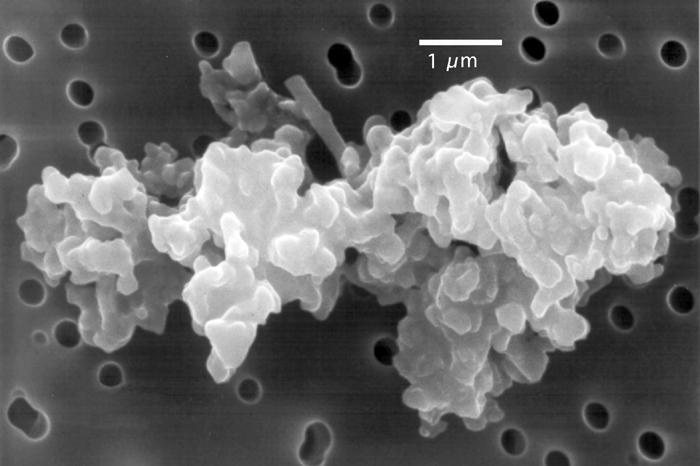
\includegraphics[width=8cm]{figures/grain.jpg}
 	\caption{A scanning electron microscopy (\textit{SEM}) image of a porous chondrite dust grain recovered from high atmosphere.  The authors of this figure are Donald E. Brownlee, University of Washington, Seattle, and Elmar Jessberger, Institut für Planetologie, Münster, Germany.
This file is licensed under CC-BY 2.5 License.}
 	\label{fig:dust_grain}
\end{figure}

\subsection{Dust density}

Bulk density of the common minerals containing the usual meteorite component elements, such as \textit{olivine}, \textit{quartz} or \textit{pyroxenes} is between $2.6 \, \si{g cm^{-3}}$ and $3.8 \, \si{g cm^{-3}}$ \citep{duda1986minerals}. A lot of interplanetary dust contains ice, which naturally has a bulk density close to $1 \, \si{g cm^{-3}}$.

The density is often assumed between $2.5 \, \si{g cm^{-3}}$ \citep{mann2014dust} and $3 \, \si{g cm^{-3}}$ \citep{mcdonnell1984cosmic}. Dust grains are often, due to photometric and historical reasons described in terms of their linear dimension $d$, which more often than not means the diameter of the sphere with the volume $V$ equivalent to the dust grain's, hence

\begin{equation}
    d = 2 \left( {\frac{3V}{4\pi}} \right)^{\frac{1}{3}} \approx 1.24 \sqrt[3]{V}.
\end{equation}

Since we meet both mass-based notation and size-based notation, it is useful to keep the conversion in mind, which stands

\begin{equation}
    m = \rho \frac{\pi}{6} d^3 \Leftrightarrow d = \sqrt[3]{\frac{6 m}{\rho \pi}},
\end{equation}

and assuming $2.5 \, \si{g cm^{-3}}$ gives

\begin{equation}
    \frac{m}{\si{kg}} \approx 1.3 \cdot 10^3 \left(\frac{d}{\si{m}}\right)^3 
\Leftrightarrow 
    \frac{d}{\si{m}} = 9 \cdot 10^{-2} \sqrt[3]{\frac{m}{\si{kg}}},
\end{equation}

which is shown in \Figref{fig:mass_size_ruler}.

\begin{figure}[h]
 	\centering
 	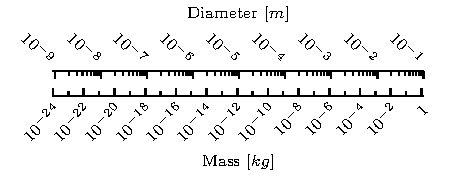
\includegraphics[width=10cm]{figures/mass_size_ruler.pdf}
 	\caption{A conversion between the mass and the diameter of a spherical dust grain, assuming the density of $2.5 \, \si{g cm^{-3}}$.}
 	\label{fig:mass_size_ruler}
\end{figure}

\section{Gravity}

TBD mention that the planets are locally relevant, but fe focus on the sun

\section{Radiation pressure}

dont forget to introduce beta factor here and how it describes effective gravity

\section{Lorentz force}

Explain charging in plasma (super quickly) and give estimates of relevance of this force, include size (mass) and time in the estimates. Mention that if the grain has a lots and lots of time, then this could be relevant

\section{Poynting-Robertson drag}

timescale estimate 

\section{Erosion}

sublimation, sputtering

\section{Collisions}

crushing law